\documentclass[11pt]{article}

\usepackage[margin=1in]{geometry}
\usepackage{mathptmx}
\usepackage[T1]{fontenc}
\usepackage[utf8]{inputenc}
\usepackage{microtype}
\usepackage{graphicx}
\usepackage{booktabs}
\usepackage{amsmath}
\usepackage{amssymb}
\usepackage{array}
\usepackage{ragged2e}
\usepackage{caption}
\usepackage{xcolor}
\usepackage[numbers,sort&compress]{natbib}
\usepackage[colorlinks=true,linkcolor=blue!45!black,citecolor=blue!45!black,urlcolor=blue!45!black]{hyperref}

\captionsetup{font=small,labelfont=bf}
\graphicspath{{figures/}}
\newcommand{\code}[1]{\texttt{#1}}

\title{\bfseries Calibration-Robust Routing as a Self-Improving Agent Harness:\\ Deploying and Evaluating Track-Record-Corrected Model Selection over the Agent Client Protocol}
\author{Teo Qing Cong Eugene\\ \small Independent \\ \small \href{https://www.linkedin.com/in/eugene-teo}{www.linkedin.com/in/eugene-teo}}
\date{\today}

\begin{document}
\maketitle

\begin{abstract}
\noindent
A multi-model coding assistant must decide, on each turn, which model should answer. The cheap-first heuristic under-serves hard turns; the always-frontier heuristic overpays on easy ones; and routing on a model's own stated confidence fails when that confidence is miscalibrated. We present a routing broker that corrects each model's self-reported confidence by a persistent, per-task-type track record before it selects the cheapest model that clears an activation barrier, and we expose the broker through the Agent Client Protocol (ACP) so it runs unmodified inside real editors \citep{acp2025}. Framed as a harness in the sense of \citet{weng2026harness}, the broker runs a plan, route, observe, and record loop over a first-class track-record store, so its routing gets cheaper and more reliable the longer it runs. On real coding-agent outcomes (three Claude tiers, eight expert tasks, ten replicates) evaluated by leave-one-replicate-out cross-validation, the corrected router retains $0.988$ completion, within $0.013$ of always-frontier, at $25.3\times$ lower cost, and it beats both naive-self-report and single-cheapest routing by $0.037$ in completion. We also report an effect that only real self-reports reveal: when a fleet's stated confidence is uniformly high, naive-self-report routing collapses into single-cheapest, and the track-record correction is precisely what restores the ability to tell hard turns from easy ones. This paper builds on the mechanism established in the companion paper \citep{teo2026cta}; here we deploy it and put it head-to-head against the baselines a routing paper is expected to beat.
\end{abstract}

\section{Introduction}

A deployed coding assistant with access to several models faces a per-turn allocation problem. Sending every turn to the strongest model is reliable but expensive. Sending every turn to the cheapest is cheap but fails the turns that need capability. Asking each model how confident it is, then routing on that answer, only works if the confidence means something. The companion paper showed, on real agents, that model self-reports are miscalibrated (Claude's are underconfident), and that a track-record correction, discounting each self-report by the model's realised pass rate on that kind of task, recovers the completion the miscalibration costs \citep{teo2026cta}.

This paper is about deployment and comparison. We make three moves.

\begin{enumerate}\itemsep2pt
\item \textbf{A protocol-native broker.} We present the router as an ACP agent that routes over a downstream fleet. On each \code{session/prompt} turn it elicits a confidence bid per candidate, corrects it by the track record, gates it, selects the cheapest model that clears the activation barrier, proxies that model's reply back to the editor, and records the outcome. Any ACP-compatible editor can use it with no bespoke integration \citep{acp2025}.
\item \textbf{A harness framing.} Following \citet{weng2026harness}, the broker is a \emph{harness}: the software around the base models that decides how they are chosen, what is remembered, and how their work is judged. Its persistent track-record store is what lets the deployed router improve across sessions rather than starting cold each time.
\item \textbf{The head-to-head.} We compare four routing policies on real agent outcomes: the corrected router, naive-self-report routing, always-frontier, and single-cheapest, reporting completion with confidence intervals, dollar cost, and the overhead of eliciting confidence.
\end{enumerate}

\section{Related work}

\paragraph{Model routing and cascades.} FrugalGPT \citep{chen2023frugalgpt} cascades from cheap to expensive models under a budget; RouteLLM \citep{ong2024routellm} learns a router from preference data. Both decide capability from features learned offline. Our router instead carries an online, per-task-type reliability estimate and corrects a \emph{live} self-report by it, so it adapts to the fleet it is actually running and improves in service. Confidence-calibrated small-large collaboration \citep{zhang2026confidence} is the closest in spirit; we differ in operating through a deployment protocol and in isolating the track-record correction as the mechanism.

\paragraph{Agent Client Protocol.} ACP \citep{acp2025} is a JSON-RPC protocol that lets any editor talk to any coding agent, in the spirit of LSP and MCP. It gives an agent an editor (buffers, terminals, diffs), where MCP gives an agent tools. ACP has no native confidence field, so eliciting one is a deliberate extension whose cost we measure.

\paragraph{Harness engineering.} \citet{weng2026harness} argues that near-term self-improvement comes from the harness around a base model, and that such loops are only as good as the signal they optimise: the evaluator is the weak link. A track-record correction plus an integrity gate is a mechanism for making a self-report-based signal trustworthy, so our router is naturally the calibration-robust evaluation layer such a harness needs. We build a component, not a full recursive-self-improvement system, and we say so. Reported failure rates for real multi-agent systems are high and driven by coordination breakdown \citep{cemri2025multiagent}, which is exactly the surface a disciplined harness is meant to reduce.

\section{The broker}

The router presents as an ACP agent to the editor and acts as a client to a downstream fleet: a routing intermediary that sits between the two. The transport-free core is a single handler, \code{AcpBroker.handle(request)}, which returns a response; a newline-delimited-JSON \code{serve()} driver hosts it for a real editor.

\paragraph{The prompt-turn loop.} On each \code{session/prompt}:
\begin{enumerate}\itemsep2pt
\item \textbf{Elicit} raw confidence bids per candidate. Two modes: \emph{prior} (a bid from a per-tier prior plus the track record, no extra turn) and \emph{probe} (a short confidence-probe turn per candidate, a real self-report at a measured cost).
\item \textbf{Gate} the raw bids (clamp to a valid confidence range; the live form of the paper's integrity gate).
\item \textbf{Correct} each bid by the model's reliability on that task type, and \textbf{select} the cheapest model whose corrected bid clears the activation barrier, escalating to the highest corrected bid if none clears.
\item \textbf{Proxy} the chosen model's \code{session/update} stream back to the editor, tagged with a routing-decision update (which model, corrected confidence, and why).
\item \textbf{Record} the realised outcome (a hidden-test pass, or a user accepting the diff) into the persistent track record, sharpening the next turn's routing.
\end{enumerate}

\paragraph{Harness properties.} The loop is the plan, route, observe, and record cycle. The track-record store (SQLite, in write-ahead-logging mode) is the persistent memory that survives across sessions. The downstream fleet is the worker pool. The difference from a plain router is that routing gets cheaper and more reliable the longer the broker runs, from its own experience, with no privileged information.

\section{Head-to-head evaluation}

\subsection{Policies}
\begin{description}\itemsep2pt
\item[CTA (corrected).] The cheapest model whose reliability-corrected self-report clears the barrier.
\item[Naive self-report.] The cheapest model whose \emph{raw} self-report clears the barrier, with no correction. This isolates what the correction buys.
\item[Always frontier.] The most capable model on every turn.
\item[Single cheapest.] The cheapest model on every turn.
\end{description}

\subsection{Method: a leave-one-replicate-out replay}
Routing is a decision over outcomes, so we evaluate it on outcomes already collected, without spending new budget. The companion paper's capability-ladder tier ran three Claude tiers (Haiku, Sonnet, Opus) on eight expert coding tasks across ten replicates, recording each run's stated confidence and hidden-test result. For each held-out replicate we estimate every model's per-task reliability and mean self-report from the \emph{other} replicates, route each task under each policy, and then look up the routed model's \emph{actual} result on the held-out replicate. No policy sees the outcome it is scored on. Averaging over the ten folds gives completion (with a bootstrap confidence interval over the folds), cost, and the head-to-head deltas. We use the unaided (\code{bare}) condition, since the agent-router comparison should turn on the model's own capability, not on the separate task-wrapper mechanism.

\subsection{Results}

\begin{table}[t]
\centering\small
\caption{Head-to-head on real agents (leave-one-replicate-out replay, expert \code{bare} tier, ten folds).}
\label{tab:h2h}
\begin{tabular}{@{}lcc@{}}
\toprule
\textbf{Policy} & \textbf{Completion (95\% CI)} & \textbf{Cost per task-set (USD)} \\
\midrule
CTA (corrected) & $0.988\;[0.963,\,1.000]$ & $0.057$ \\
Naive self-report & $0.950\;[0.913,\,0.988]$ & $0.024$ \\
Always frontier & $1.000\;[1.000,\,1.000]$ & $1.440$ \\
Single cheapest & $0.950\;[0.913,\,0.988]$ & $0.024$ \\
\bottomrule
\end{tabular}
\end{table}

\begin{figure}[t]
\centering
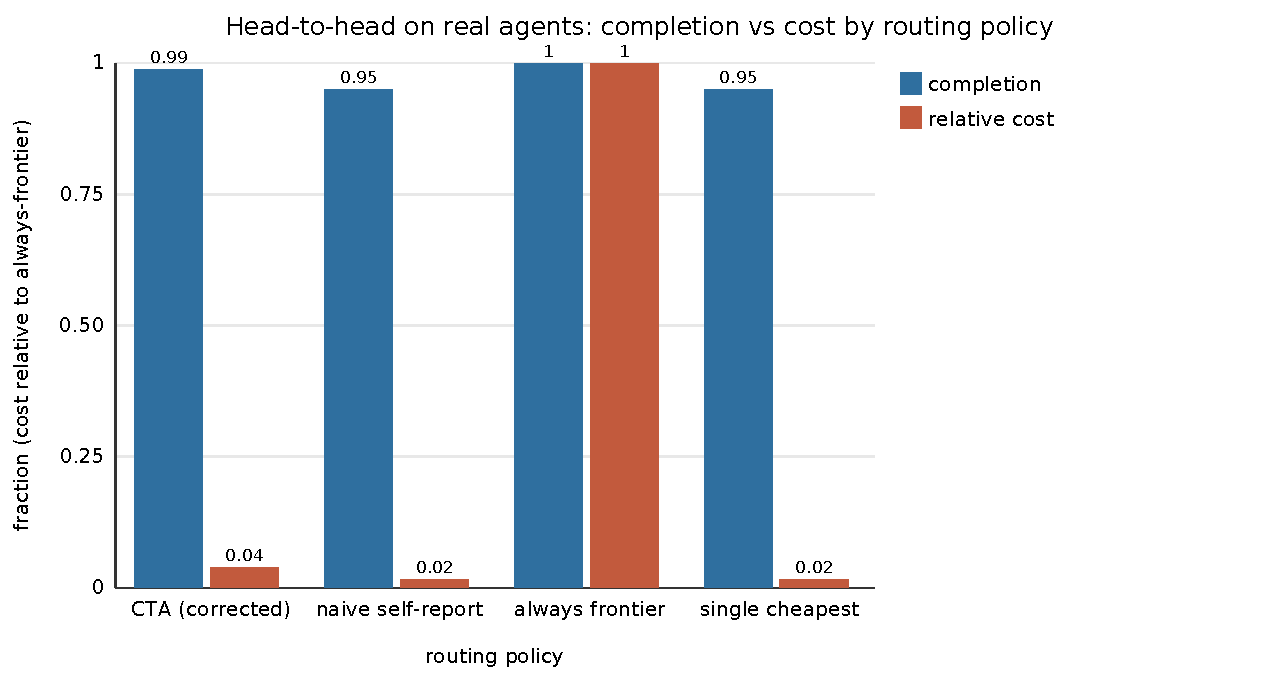
\includegraphics[width=0.86\linewidth]{headtohead.pdf}
\caption{Completion against cost by routing policy, cost shown as a fraction of the always-frontier cost. The corrected router keeps almost all of the frontier's completion at a small fraction of its cost, and it separates from naive-self-report and single-cheapest, which sit together.}
\label{fig:h2h}
\end{figure}

Table~\ref{tab:h2h} and Figure~\ref{fig:h2h} give the result. The corrected router retains $0.988$ completion, within $0.013$ of always-frontier, at $\mathbf{25.3\times}$ lower cost, and it beats naive-self-report and single-cheapest by $\mathbf{+0.037}$ in completion. The gap is modest here because Haiku is already strong on these tasks ($0.950$ unaided); the mechanism spends the frontier only on the roughly one turn in twenty a cheap model actually fails, which is exactly where it should.

\paragraph{An effect only real self-reports reveal.} Naive-self-report routing scores identically to single-cheapest. Claude's stated confidence is uniformly high (around $0.9$) and always clears the barrier, so routing on the raw bid always picks the cheapest model. Without the track-record correction, self-report routing carries no information that distinguishes hard turns from easy ones; the correction is what restores that information. This is a sharper statement of the companion paper's calibration thesis, and it only appears when the self-reports are real rather than synthetic.

\subsection{A live end-to-end vignette}
To show the broker running as a deployed system rather than a replay, we ran it
live over four real Claude subagent turns, with the track record warm-started from
the ladder calibration (Table~\ref{tab:vignette}, Figure~\ref{fig:vignette}). Each
turn, the broker elicited a bid, corrected it, routed to the chosen model, and had
that real model solve the task against hidden tests. Three tasks routed to the cheap
model (Haiku) and passed. The fourth, \code{is\_match}, is the one task Haiku is
unreliable on (ladder reliability $0.70$): its corrected bid falls to $0.595$, below
the $0.70$ barrier, so the broker escalated to Sonnet, which passed. The routed
spend was $\$0.045$ against $\$0.72$ for always-frontier, a $16\times$ saving on
this short run, and every turn passed. The broker protected completion exactly where
the cheap model was weak and paid the cheap price everywhere else.

\begin{table}[t]
\centering\small
\caption{Live ACP-broker vignette over four real Claude subagent turns. Corrected
bids are Haiku/Sonnet/Opus; the cheapest model clearing the $0.70$ barrier wins.}
\label{tab:vignette}
\begin{tabular}{@{}llccc@{}}
\toprule
\textbf{Turn} & \textbf{Task} & \textbf{Routed to} & \textbf{Corrected bids (h/s/o)} & \textbf{Outcome} \\
\midrule
1 & \code{fraction\_to\_decimal} & Haiku & $0.85 / 0.92 / 0.96$ & pass \\
2 & \code{multiply\_strings} & Haiku & $0.85 / 0.92 / 0.96$ & pass \\
3 & \code{word\_break} & Haiku & $0.85 / 0.92 / 0.96$ & pass \\
4 & \code{is\_match} & Sonnet & $0.595 / 0.92 / 0.96$ & pass \\
\bottomrule
\end{tabular}
\end{table}

\begin{figure}[t]
\centering
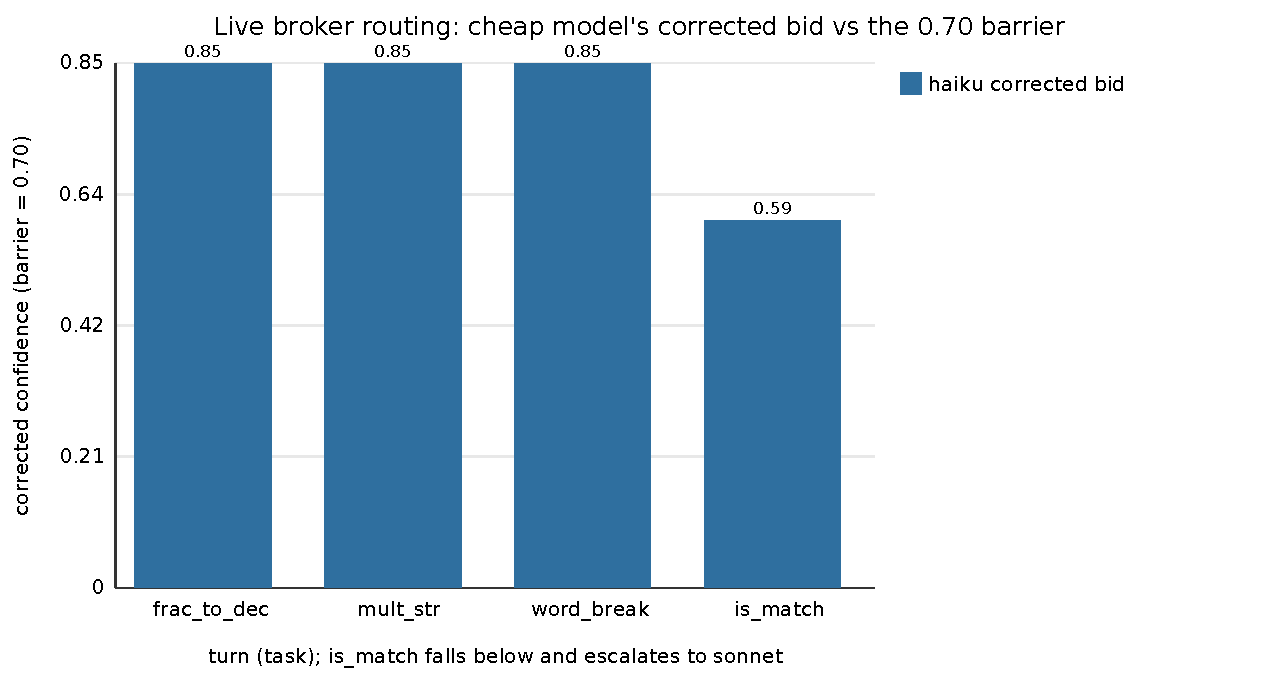
\includegraphics[width=0.80\linewidth]{vignette_routing.pdf}
\caption{The cheap model's (Haiku) reliability-corrected bid across the four live
turns. It clears the $0.70$ barrier on the first three tasks, which route to Haiku,
and dips to $0.595$ on \code{is\_match}, which escalates to Sonnet. The dip below the
barrier is the escalation.}
\label{fig:vignette}
\end{figure}

\subsection{Probe overhead}
Eliciting a live confidence bid costs one short probe turn per candidate; the static policies (always-frontier, single-cheapest) pay none. In the harness we account this separately and report it as a fraction of the total cost. On a three-model fleet with short probes it stays a small fraction of the solve cost. The track-record correction needs no probe once a record exists, so a deployment can fall back to prior mode as the record accrues.

\section{Limitations}
\begin{itemize}\itemsep2pt
\item \textbf{Failure-contingent advantage.} The completion gain is bounded by how often the cheap model actually fails. On a suite where a cheap model is already reliable, the correction is a cost win with no completion regression, not a completion win. We report the honest $0.037$.
\item \textbf{Underconfident fleet.} Claude self-reports are underconfident on standard tasks, so the overconfident failure mode that most rewards correction is not sourceable from this fleet without contrived tasks; we do not manufacture it. A fleet with a genuinely overconfident member would widen the gap.
\item \textbf{Protocol youth.} ACP is recent and its remote transport is still in progress; we pin a spec version and stay on local stdio.
\item \textbf{A component, not an RSI system.} The broker is the calibration-robust routing and memory layer of a harness, not a self-rewriting agent.
\end{itemize}

\section{Conclusion}
Correcting a live self-report by a persistent track record turns an unreliable routing signal into a useful one, and doing it inside a deployment protocol makes the resulting router usable in real editors while it improves in service. On real agent outcomes the corrected router buys most of the frontier's reliability at a fraction of its cost, and it is the correction, not the self-report, that does the work.

\bibliographystyle{plainnat}
\bibliography{refs}

\end{document}
